\chapter{Extended source in SEM3D}

A number of modifications are applied to SEM3D code to implement the extended-source model. These changes are detailed in Chapter \ref{chapmodi}. Here, instructions for extended-source modeling in this new version of SEM3D code are explained. \\


The only changes apply to the 'input.spec' file. The user should define a block of 'extended source' as shown in Figure \ref{sem}: \\


% FIGURE : convert_moment
\begin{center}
\leavevmode
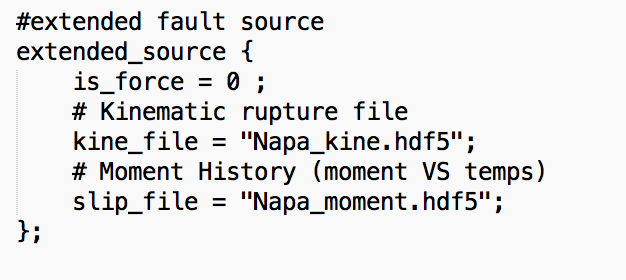
\includegraphics[scale=0.5]{figures/input-moment.png} 
\captionof{figure}{Extended source block in input.spec file for moment option.}
\label{sem} 
\vspace{1cm}
\end{center}



The first necessary information in 'extended source' block is the choice of force or moment-time history for the extended-source model. Here, we show the example of Napa bedrock case where we calculate moment-time history so that 'is\textunderscore force' parameter is set to 0. For force option, it should be set to 1. \\


Second, the name of file containing source properties such as coordinates should be given for 'kine\textunderscore file'. \\

Last, the name of file where moment-time history (or force-time history for force option) is stocked is specified as 'slip\textunderscore file'.


For Napa example, we provide the folder 'SEM\textunderscore extended\textunderscore source\textunderscore Napa\textunderscore rocher' folder. Even though we use a realistic model of fault plan, for simplicity, we prefer to define a single  type of soil in the propagation media. Once the simulation terminates, the procedure to analyze the outputs remain exactly the same as before. \\

















 